\documentclass[border=1pt, tikz]{standalone}
\usepackage[rm]{roboto}
%\usepackage[rm,light]{roboto}

\usetikzlibrary{positioning, fit, decorations.text}
%\tikzset{every picture/.style={/utils/exec={\sffamily}}}
\tikzset{every picture/.style={line width=1pt}}

\definecolor{kts-blue}{RGB}{237,241,251}

\begin{document}
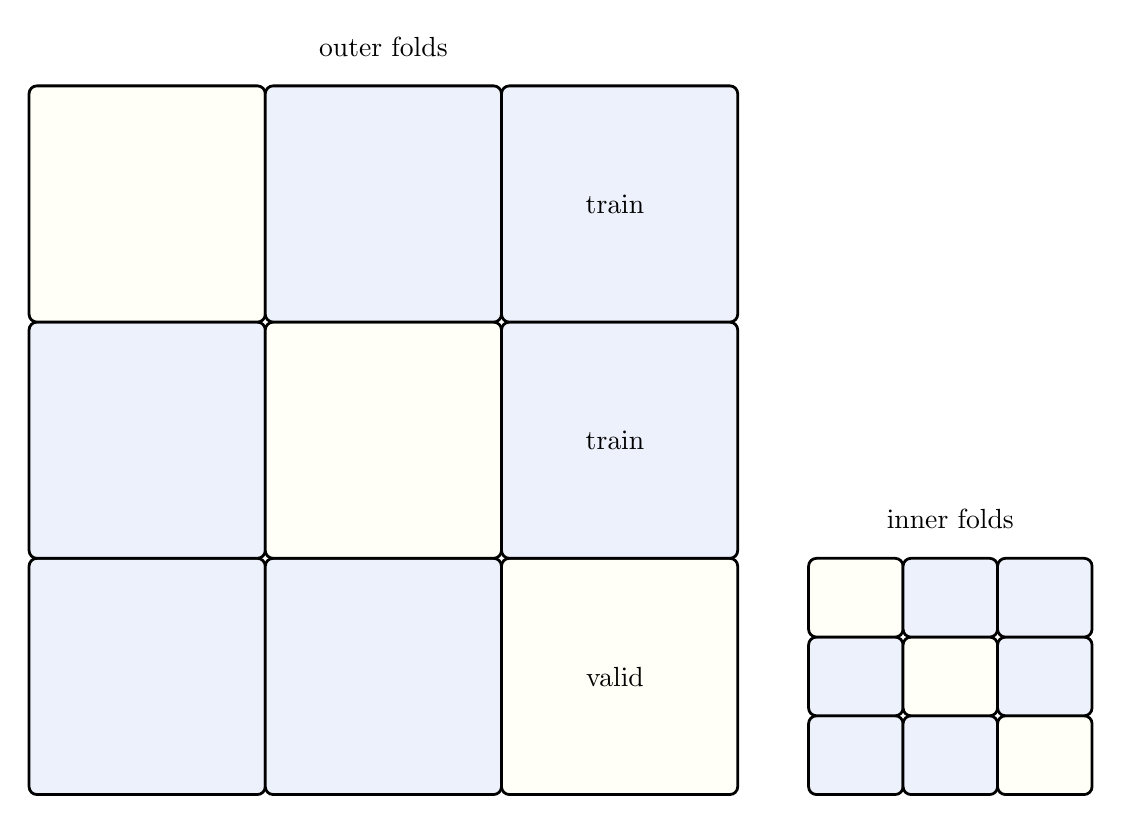
\begin{tikzpicture}
    [rect/.style = {rectangle, draw, align=center, 
            inner xsep=6mm, inner ysep=3mm, fill=kts-blue, rounded corners=0.1cm},
    -latex,     
    fs/.style = {rectangle, draw, align=center, 
            rounded corners=0.1cm},
    -latex,  
    ]
    

\node (t) at (-3, 8) {outer folds};
\node (t) at (4.2, 2) {inner folds};
%\node[rect, minimum height=3cm, minimum width=3cm, fill=yellow!3] (n) at (0, 0) { valid };
%\node[rect, minimum height=3cm, minimum width=3cm] (n) at (0, 3) { train };
%\node[rect, minimum height=3cm, minimum width=3cm] (n) at (0, 6) { train };
%\node[rect, minimum height=1cm, minimum width=1cm, fill=yellow!3] (n) at (3, -1) {  };
%\node[rect, minimum height=1cm, minimum width=1cm] (n) at (3, 0) {  };
%\node[rect, minimum height=1cm, minimum width=1cm] (n) at (3, 1) {  };


\node[rect, minimum height=3cm, minimum width=3cm] (n) at (-6, 0) {  };
\node[rect, minimum height=3cm, minimum width=3cm] (n) at (-6, 3) {  };
\node[rect, minimum height=3cm, minimum width=3cm, fill=yellow!3] (n) at (-6, 6) {  };
\node[rect, minimum height=3cm, minimum width=3cm] (n) at (-3, 0) {  };
\node[rect, minimum height=3cm, minimum width=3cm, fill=yellow!3] (n) at (-3, 3) {  };
\node[rect, minimum height=3cm, minimum width=3cm] (n) at (-3, 6) {  };
\node[rect, minimum height=3cm, minimum width=3cm, fill=yellow!3] (n) at (0, 0) { valid };
\node[rect, minimum height=3cm, minimum width=3cm] (n) at (0, 3) { train };
\node[rect, minimum height=3cm, minimum width=3cm] (n) at (0, 6) { train };
\node[rect, minimum height=1cm, minimum width=1cm] (n) at (3, -1) {  };
\node[rect, minimum height=1cm, minimum width=1cm] (n) at (3, 0) {  };
\node[rect, minimum height=1cm, minimum width=1cm, fill=yellow!3] (n) at (3, 1) {  };
\node[rect, minimum height=1cm, minimum width=1cm] (n) at (4.2, -1) {  };
\node[rect, minimum height=1cm, minimum width=1cm, fill=yellow!3] (n) at (4.2, 0) {  };
\node[rect, minimum height=1cm, minimum width=1cm] (n) at (4.2, 1) {  };
\node[rect, minimum height=1cm, minimum width=1cm, fill=yellow!3] (n) at (5.4, -1) {  };
\node[rect, minimum height=1cm, minimum width=1cm] (n) at (5.4, 0) {  };
\node[rect, minimum height=1cm, minimum width=1cm] (n) at (5.4, 1) {  };


\end{tikzpicture}
\end{document}